\chapter{The PyBayes Library}

In this chapter the PyBayes library that is being developed with the aim to fulfil the requirements
posed in the previous chapter (p. \pageref{sec:Requirements}) is presented. After a brief introduction
the library design, which builds on the performed software analysis, is shown and discussed.
Various development practices used are later examined and the chapter is concluded by a performance
comparison of various implementations of the Kalman filter (from PyBayes and BDM) benchmarked under
4 different implementation environments.

\section{Introduction to PyBayes}

PyBayes\footnote{the name PyBayes had been previously used for an unrelated project dealing with
Bayesian networks by Denis Deratani Maua, who later proclaimed the project dead and allowed us
to use the name.}
is a Python/Cython library for recursive Bayesian estimation actively developed by the
author of this text, a result of the software analysis carried-out. The development happens publicly
and openly using the git\footnote{\url{http://git-scm.com/}} version control system on the
GitHub\footnote{\url{http://github.com}} source-code hosting service at the address
\url{http://github.com/strohel/PyBayes} that also serves as the home page of the project; PyBayes is
also accessible from the Python Package Index (PyPI).\footnote{\url{http://pypi.python.org/pypi/PyBayes}}
\ifattachements
	Additionally, the snapshot of version 0.3 is available on the enclosed CD-ROM.
\fi
PyBayes is a free/open-source software licensed under the GNU GPL\footnote{GNU General Public
License: \url{http://www.gnu.org/licenses/gpl.html}}, version 2 or later. Version 0.3 of PyBayes is
described in this text; we expect PyBayes to evolve in future and thus some claims present this
chapter may become outdated. All currently planned future changes are however mentioned at
appropriate places.

The goal of PyBayes is to provide a Python library that satisfies the posed requirements, is very
convenient to develop with even when prototyping novel algorithms, but fast enough to be deployed in
production. Library design should be object-oriented and very clean to be well comprehensible.
In order to achieve both of these usually contradicting demands, PyBayes uses a special
technique where the same source code can be interpreted by Python as usual (giving all advantages
of Python) or compiled using Cython which makes use of additional \emph{augmenting files} that are present
in sources to provide static
type declarations to performance-critical code-paths; PyBayes thus employs Cython's \emph{pure Python
mode}. The Cython build is currently 50\% to 200\% faster than Python depending on the algorithm and
level of optimisation applied to it, see \autoref{sec:PyBayesPerformance} (p.~\pageref{sec:PyBayesPerformance})
for example measurements. PyBayes' \verb|setup.py|, the use of which is the standard way to install
Python packages, automatically detects whether Cython is installed on the system and uses it when
possible. NumPy's \verb|ndarray| (N-dimensional array) of Python \verb|floats|\footnote{Python
\verb|float| (\verb|numbers.Real|) corresponds to C \verb|double|} is used as principal
numeric type for vectors and matrices for its low overhead, convenience and interoperability.

PyBayes sources are maintained to be compatible with Python versions 2.5, 2.5 and 2.7; Python 3
compatibility can achieved using the 2to3\footnote{\url{http://docs.python.org/library/2to3.html}}
automatic code conversion tool, the sources are kept to be convertible without interaction
(CPython's \verb|-3| command-line can be used for this task). To promote code readability, coding
style prescribed by the PEP 8\footnote{Python Enhancement Proposal 8:
\url{http://www.python.org/dev/peps/pep-0008/}} is followed when feasible.

The sections below present the library design and explain some decisions taken during development;
they complement the \textbf{PyBayes API Documentation}, which is a reference guide intended for
PyBayes users. API Documentation is available on-line at \url{http://strohel.github.com/PyBayes-doc/}%
\ifattachements%
\ and on the enclosed CD-ROM%
\fi%
.

All class diagrams in this text utilise standard UML\footnote{Unified Modelling Language:
\url{http://www.uml.org/}} notation and are not an exhaustive reference of all classes, members and
methods --- they rather illustrate the API Documentation; inherited attributes and methods are not
shown in diagrams. Unless noted otherwise, all references to
files and folders in this chapter refer to the respective files/folders in the PyBayes source code
repository.\footnote{\url{http://github.com/strohel/PyBayes}} Python software nomenclature is used,
most notably the following terms:
\begin{description}
	\item[module] a file with .py extension (but denoted without it) that contains Python code and
		has its own namespace.
	\item[package] a folder that contains above modules and possibly other packages; package
		namespace is identical with its \verb|__init__| module that has to be present.
\end{description}

\section{Library Layout}

The source code of PyBayes is arranged as follows:

\noindent\begin{tabular}{rp{\textwidth-92pt}}
\verb|doc/|      & control files for generating documentation (see also \autoref{sec:PyBayesDocsTests}). \\
\verb|examples/| & auxiliary scripts and benchmark sources. \\
\verb|pybayes/|  & PyBayes Python package; the actual implementation is located in this package. \\
\verb|scratch/|  & miscellaneous and temporary files. \\
\verb|thesis/|   & source code of this text. \\
\verb|tokyo/|    & source code of the Tokyo project, bundled with PyBayes (see \autoref{sec:PyBayesWrappers}). \\
\verb|COPYING|   & the text of GNU GPL v2, the PyBayes license. \\
\verb|HACKING.rst| & a guide for PyBayes developers; can be viewed as plain-text. \\
\verb|README.rst|  & general information and installation instructions. \\
\verb|setup.py|    & setup script, a tool to build and install PyBayes. \\
\end{tabular}

The \verb|pybayes| package, the most important part that forms the actual PyBayes library, contains
3 supportive packages that are considered private to PyBayes (that may change without notice), and
2 following modules that form the public API of the library (overview shown in \autoref{fig:DiaPyBayes}):
\begin{description}
	\item[pdfs] module contains a framework of {\pdfs} and related classes.
	\item[filters] module contains Bayesian filters.
\end{description}

All classes mentioned in this chapter are \emph{Cython extension classes} in the Cython build of
PyBayes (for smaller overhead) and ordinary Python classes in the Python ``build``.

\begin{figure}[h]
	\centering
	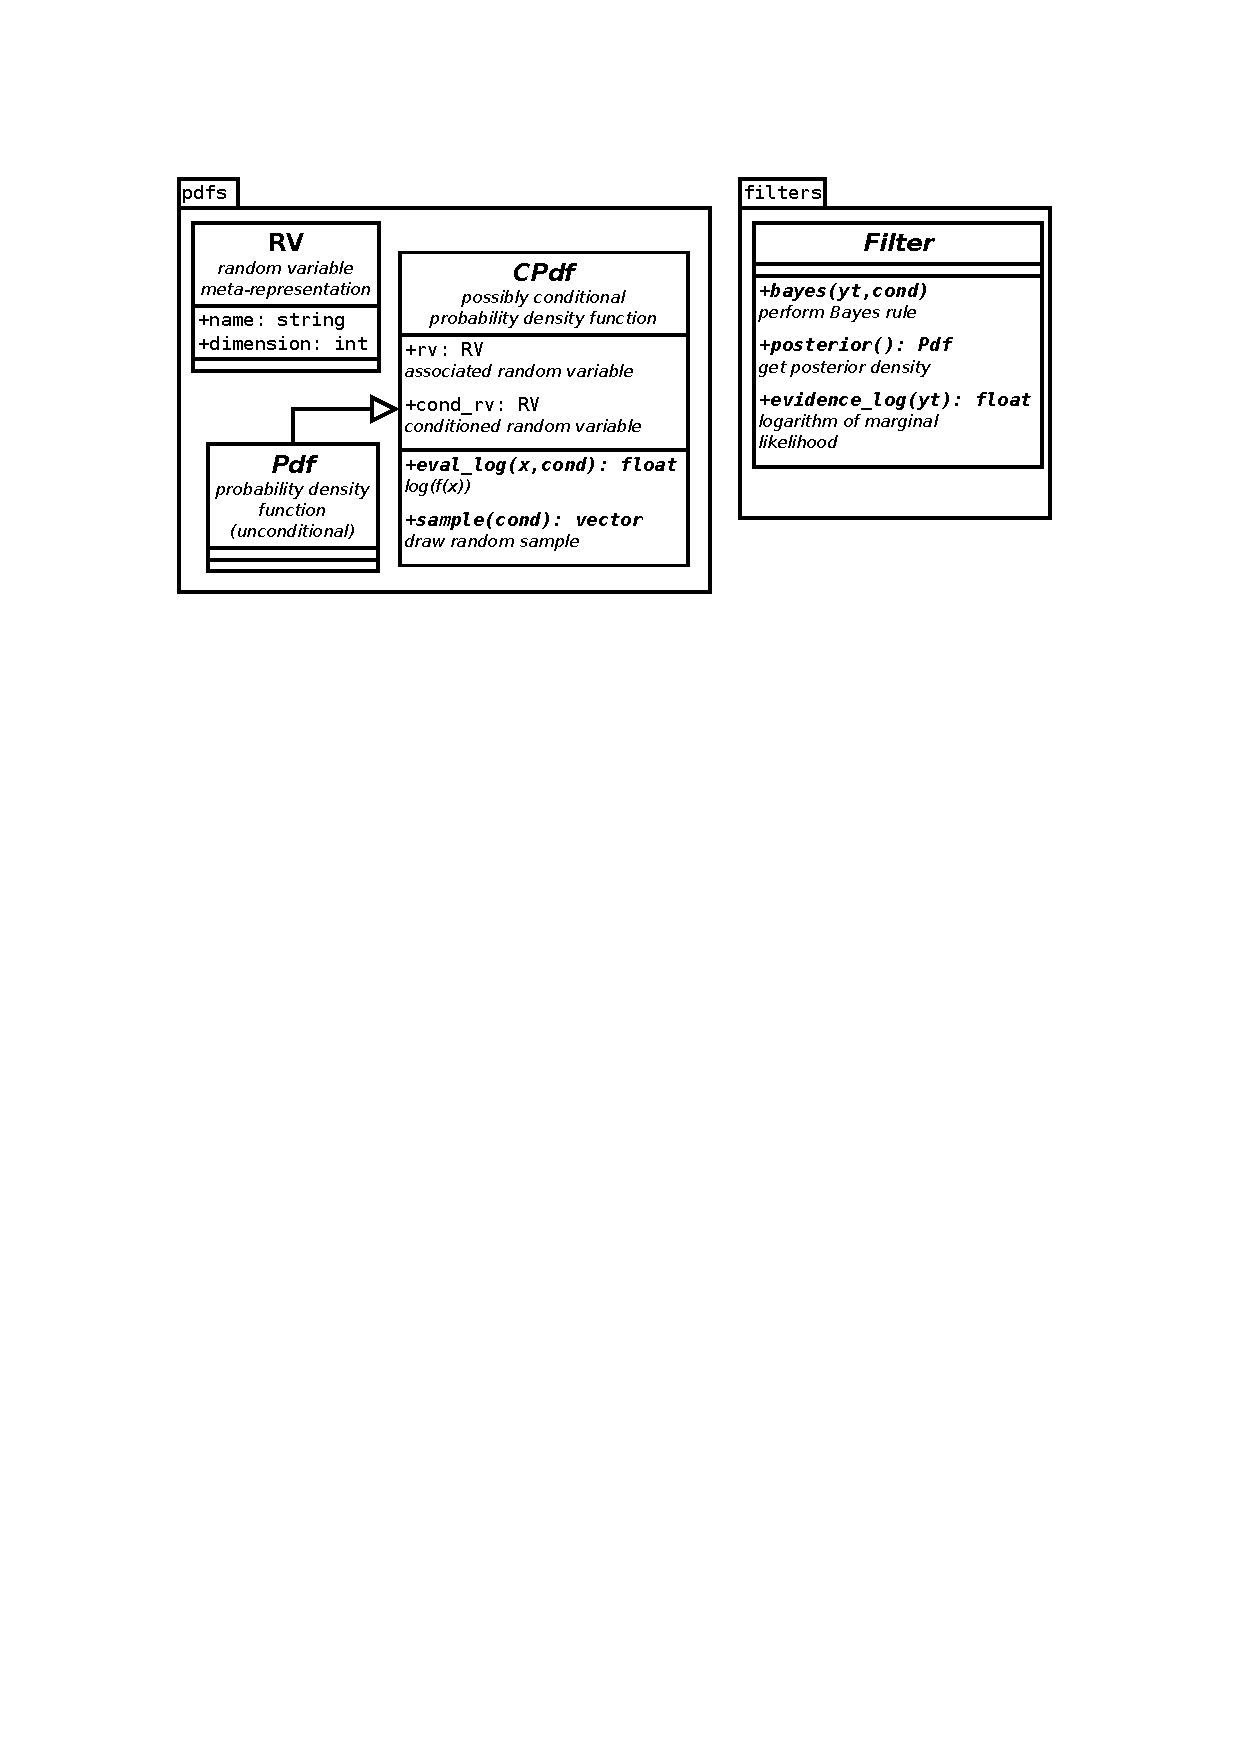
\includegraphics[width=\textwidth,keepaspectratio=true,clip=true,trim=3cm 196mm 3cm 3cm]{./diagrams/PyBayes.pdf}
	\vspace{-8mm}
	\caption[High-level overview of the PyBayes library]{High-level overview of the PyBayes library;
	simplified}
	\label{fig:DiaPyBayes}
\end{figure}

\subsection{Probability Density Functions}

Probability density functions have central role in the theory of Bayesian filtering and thus should
receive great attention during library design. Probability density functions should be both flexible
and lightweight as copying them is needed for example in the marginalized particle filter. In PyBayes
{\pdfs} are multivariate (even distributions that cannot be generalised to multiple dimensions take
singe-valued vectors as parameters for consistency and easier static typing).

2 basic categories of {\pdfs} can be distinguished from the implementation point of view:
unconditional ones whose statistics are fixed once the distribution is constructed and conditional
{\pdfs} whose statistics depend on a free parameter; depending on one's standpoint, unconditional
{\pdfs} may be viewed as a subclass of unconditional ones (that would have additional method
\verb|set_condition(cond)| or similar) or the other way around where unconditional {\pdf} is viewed
as a specialisation of the conditional ones with a restriction that condition is empty.
The latter approach is used by PyBayes for being less error-prone in our belief.
Alternatively, conditional and unconditional densities could be unrelated (impractical in our case)
or unified in one class without specifying conditionality (in fact, PyBayes is not far from this).

All {\pdfs} are represented using an abstract class \emph{CPdf} that provides interface for querying
random variable and conditioning variable dimensions (methods \verb|shape()| and \verb|cond_shape()|),
for computing expected value and variance (methods \verb|mean()| and \verb|varience()|) that take
condition as a parameter, for computing natural logarithm of the {\pdf} value in a given point
(\verb|eval_log()|) and for drawing random samples (\verb|sample()|), both also accepting condition
in parameters. A few support methods for use by subclasses not are provided to reduce code
duplication, these aren't discussed here. The CPdf class also holds references to random variable
and conditioning variable descriptions (attributes \verb|rv| and \verb|cond_rv|) which are talked 
bout in the next chapter. By convention \verb|rv| and \verb|cond_rv| to a valid \emph{RV} object
that can, however, signify ``empty random variable''.

\begin{figure}[h]
	\centering
	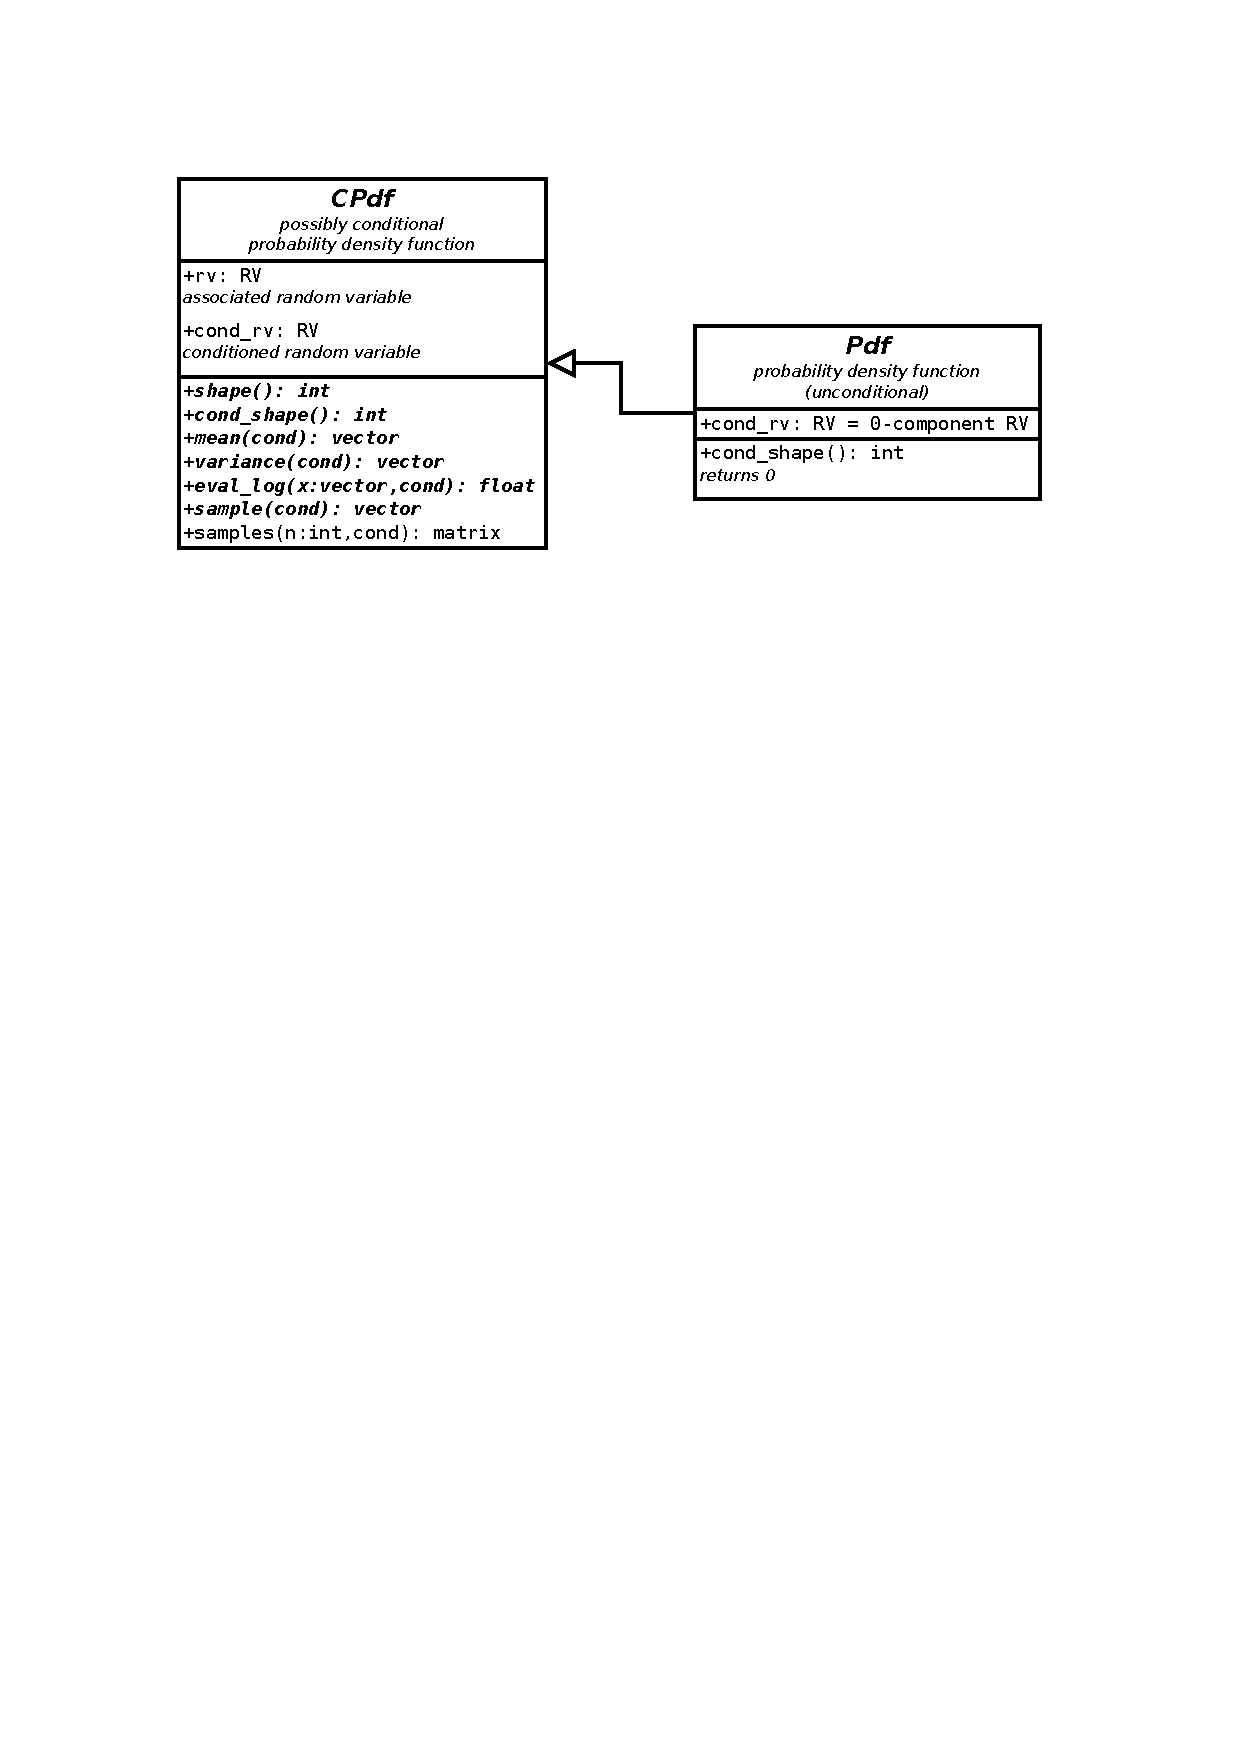
\includegraphics[width=\textwidth,keepaspectratio=true,clip=true,trim=3cm 204mm 3cm 3cm]{./diagrams/pdfs.pdf}
	\vspace{-8mm}
	\caption{Class diagram of the {\pdf} prototypes}
	\label{fig:DiaPdfs}
\end{figure}

The \emph{Pdf} is a very thin subclass of CPdf providing an implementation of the \verb|cond_shape()|
that returns zero to signify empty condition; by convention, Pdf subclasses also should set
\verb|cond_rv| to ``empty random variable''. The function of the Pdf class is therefore rather
semantic than technical distinction between conditional and unconditional {\pdfs}.

Outline of {\pdf} prototypes is shown in the \autoref{fig:DiaPdfs}.

\subsection{Random Variable Meta-representation}

In mathematics, the relation between random variables and {\pdfs} is follows: a {\pdf} is associated
to a random variable, e.g. ``random variable \(X\) is normally distributed''. This is impractical in
software (should drawing a million bare samples produce a million copies of a random variable?) but
let us show that the relation between random variables and {\pdfs} couldn't be entirely dropped
without a substitution, let's look at that following example.

The chain rule for {\pdfs} is heavily used in Bayesian filtering and should be adequately supported
by software. While simple cases can be represented without problems, when for example
\(p(\mathbf{a},\mathbf{b}|\mathbf{c},\mathbf{d})\)
from \eqref{eq:ProdCPdfExample} is desired to be represented, additional information have to be
supplied by the user (programmer) so that the implementation ``knows'' how and what parts of involved
vectors are passed to underlying densities \(p_1\) and \(p_2\). The implementation wouldn't be able
to guess evaluation order, order of components in \(p_1\) condition etc. without such additional
information.
\begin{align}
	p(\mathbf{a},\mathbf{b}|\mathbf{c},\mathbf{d}) &=
		p_1(\mathbf{a}|\mathbf{c},\mathbf{b}) p_2(\mathbf{b}|\mathbf{d}) \label{eq:ProdCPdfExample} \\
	\mathbf{z} &= (\mathbf{a}, \mathbf{b}, \mathbf{c}, \mathbf{d}) =
		(a_1, a_2, b_1, b_2, c_1, c_2, d_1, d_2)  \label{eq:ProdCPdfCombinedVec}
\end{align}

In software it is practical to combine both random and conditioning variable
of the left hand side of \eqref{eq:ProdCPdfExample} into one vector; let \(\mathbf{z}\)
\eqref{eq:ProdCPdfCombinedVec} denote such vector (\(\mathbf{a}, \mathbf{b}, \mathbf{c}, \mathbf{d}\)
are thus all two-dimensional). Now suppose that
the implementation has to pass the vector representing condition \((\mathbf{c}, \mathbf{b})\) to
the distribution \(p_1\) assuming that \(p_2\) was already evaluated. The problem that the software
must solve therefore reduces to the task of finding indexes of the \((\mathbf{c},\mathbf{b})\)
components within vector \(\mathbf{z}\); the solution is indeed an index vector \((5,6,3,4)\),
assuming one-based indexing.

The first option of passing such information from the user to the implementation would be to force
her to specify the relations between distributions manually
using index vectors (or a similar measure) directly; we believe that it is however error-prone
and inconvenient. The other method is to make a symbolic association between {\pdfs} and random
variable descriptions, but the other way around --- {\pdfs} would ``contain'' the description of
random variables they make use of, in our example above \(p_1\) would contain an information
that it is associated with random variable \((\mathbf{a}\)) and conditioning variable
\((\mathbf{c},\mathbf{b})\).

The second approach is used in PyBayes even though it brings some computational overhead (that we
think is worth the simplicity it brings). As mentioned in the previous section, the CPdf class has
\verb|rv| and \verb|cond_rv| attributes that hold instances of the RV class. Simply put, the concept
of random variable meta-representation can be viewed as a kind of \emph{semantic}, or \emph{symbolic
indexing} that should make the life of the PyBayes user easier.

The \emph{RV} class is essentially a list of ``random variable components'' represented using the
RVComp objects. RV provides a few methods to test relationships between 2 random variables
(whether a RV is subset of another RV etc.) and one notable method, \verb|indexed_in()| (that happen
to be shown in the \autoref{fig:Coverage} on page \pageref{fig:Coverage}). Suppose
that RV \(x\) has components \((x_1, x_2, \dotsc, x_n)\) and RV \(y\) is a subset of \(x\) and contains
components \((x_{i_1}, x_{i_2}, \dotsc, x_{i_m})\); \verb|y.indexed_in(x)| then returns an index array
\((i_1, i_2, \dotsc, i_m)\) which is suitable for NumPy array indexing methods.\footnote{the notation
used here is simplified; actual implementation allows for multivariate components \(x_i\) --- \(i_j\)
in returned index array are therefore ranges of integers.}

The \emph{RVComp} class is a simple container for the \verb|dimension| (which must be greater than
zero) and \verb|name| (which is optional) attributes; RV caches aggregate name and dimension. An
important principle in PyBayes is that RVComp comparisons are \emph{instance-based}: 2 RVComp
objects are considered equal if and only if they refer to the same instance.\footnote{the name
attribute thus serves only for aesthetic purposes.} This is fast (compared to for example
name-based equality), saves memory, prevents collisions and is convenient in Python thanks to its
call-by-object semantics. The effects are best demonstrated in the following recording of an
interactive Python session:

\begin{Verbatim}[samepage=true,gobble=1,label=RV and RVComp demonstration,frame=single]
	>>> rv = RV(RVComp(1, "a"))
	>>> rv.contains(RVComp(1, "a"))
	False

	>>> a = RVComp(1, "pretty name")
	>>> b = RVComp(1, "pretty name")  # same name, different instance
	>>> rv = RV(a)
	>>> rv.contains(a)
	True
	>>> rv.contains(b)
	False
\end{Verbatim}
A RVComp without a name (with \verb|name| attribute set to None), that can be called \emph{anonymous
component}, is created in CPdf when the user doesn't pass RV to the constructor, but is otherwise
insignificant.

\begin{figure}[ht]
	\centering
	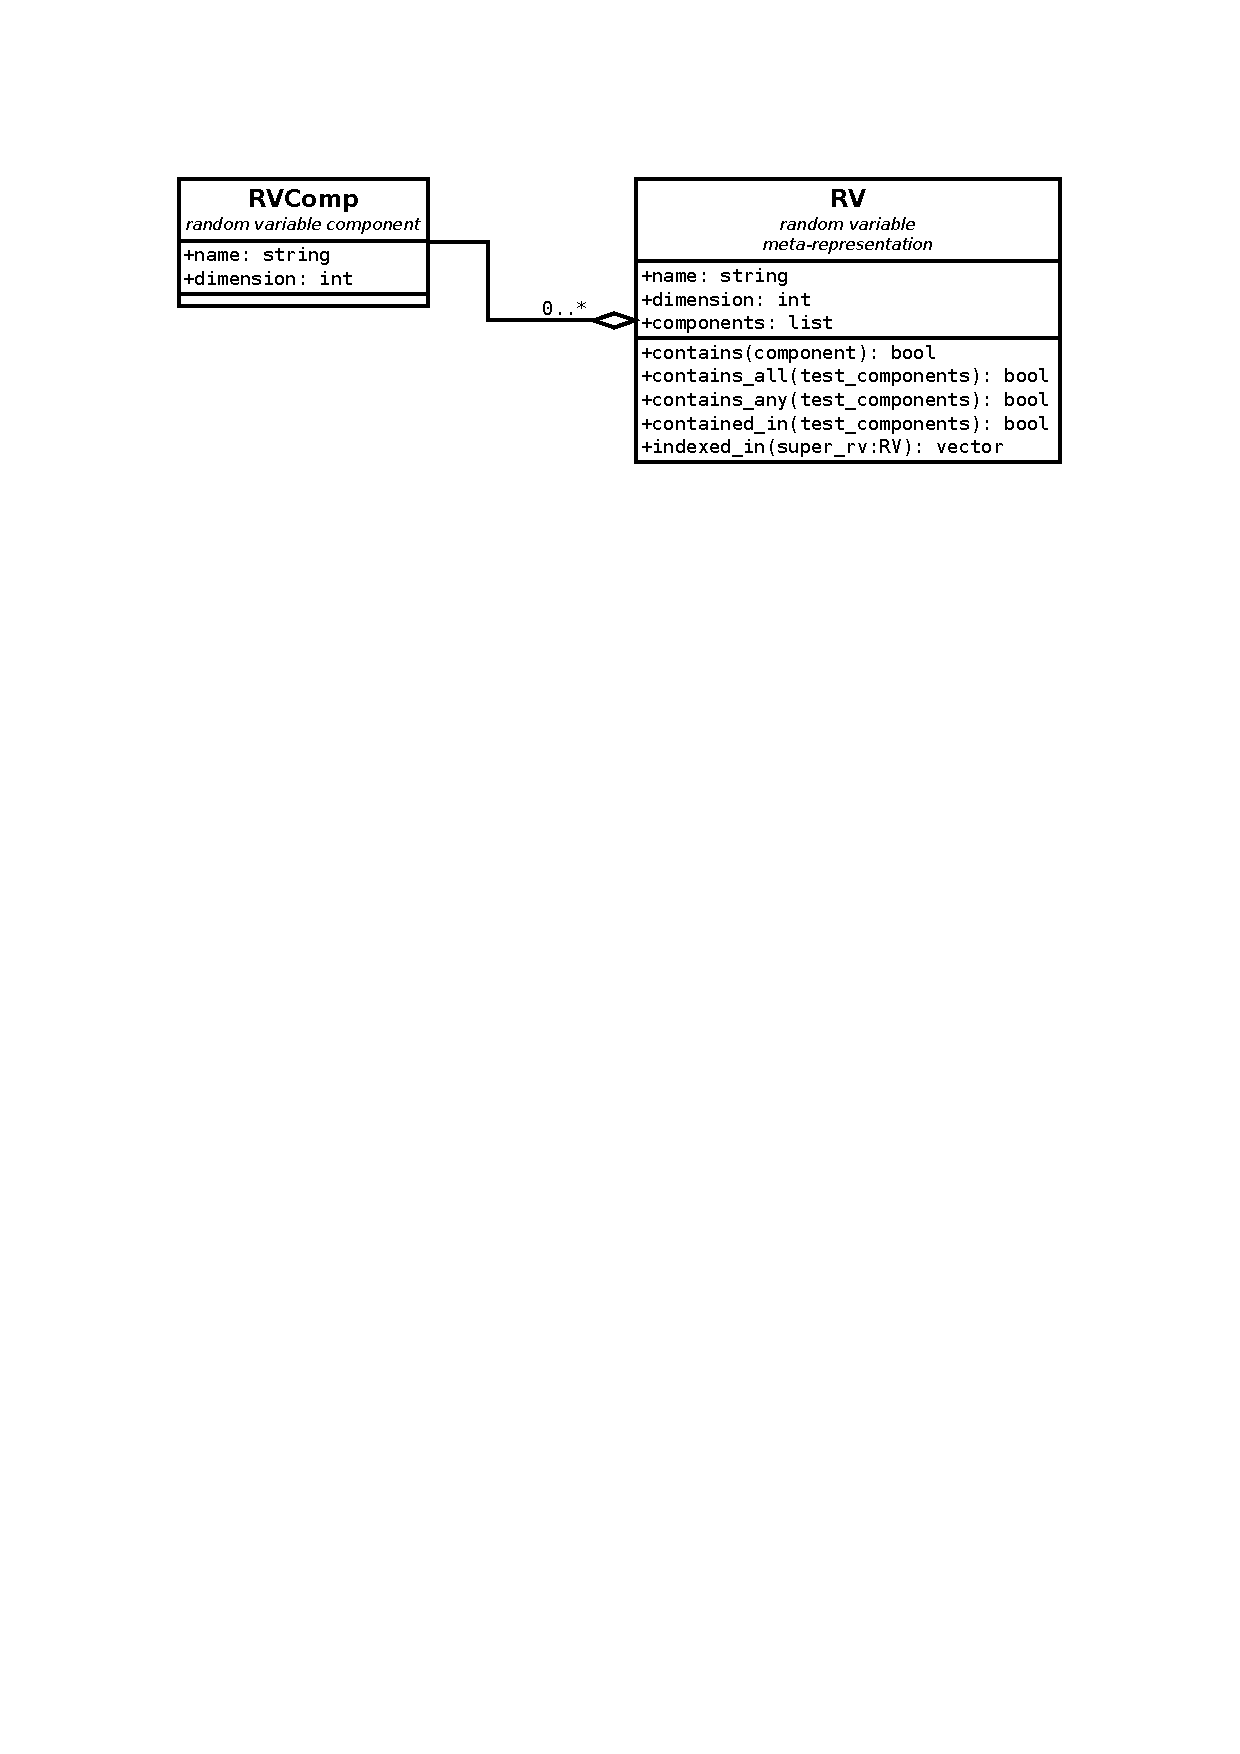
\includegraphics[width=\textwidth,keepaspectratio=true,clip=true,trim=3cm 218mm 3cm 3cm]{./diagrams/rvs.pdf}
	\vspace{-8mm}
	\caption{Class diagram of the random variable framework}
	\label{fig:DiaRvs}
\end{figure}

The concept of random variables might be used also for some Bayesian filters in future should there
be a need for it. On the other hand, documented conventions (such as ordering of vector components)
are used rather than RVs where feasible. Overview of RV and RVComp classes can be seen in the
\autoref{fig:DiaRvs}.

\subsection{Gaussian Probability Density Functions}

We continue by a brief mention of implemented {\pdfs}; our policy is to add new distributions on
as-needed basis rather than trying to have exhaustive set from the beginning. Every user of
PyBayes can create its own distributions by subclassing Pdf of CPdf and implementing meaningful
methods (there is no requirement for implementing unused methods).

PyBayes ships standard multivariate normal (Gaussian) {\pdf} through the \emph{GaussPdf} class;
related log-normal {\pdf} \emph{LogNormPdf} is also provided and shares common abstract superclass,
\emph{AbstractGaussPdf} with GaussPdf. The AbstractGaussPdf class only holds mean attribute \verb|mu|
and covariance matrix attribute \verb|R| and is useful mainly for the family of conditional Gaussian
{\pdfs} described below.

The most general conditional Gaussian distribution is the \emph{GaussCPdf} class that takes two
functions \verb|f| and \verb|g| as parameters\footnote{currently any Python callable objects are
accepted; NumPy \verb|ufunc| class will be evaluated for suitability in future.}
plus the optional \verb|base_class| parameter in
constructor. The \verb|base_class| parameter defaults to GaussPdf, but can be set tu LogNormPdf (to
any AbstractGaussPdf subclass in general); the base class parameter determines resulting density ---
both conditional normal and log-normal distributions can be obtained without any code duplication,
thanks to abstraction provided by AbstractGaussPdf. GaussPdf transforms supplied condition \(c\)
using \eqref{eq:GaussCPdf}, substitutes to AbstractGaussPdf and calls respective \verb|base_class|
method.
\begin{equation} \label{eq:GaussCPdf}
	\begin{aligned}
		\mu &= f(c) \\
		R &= g(c)
	\end{aligned}
\end{equation}

First specialisation of GaussCPdf is the \emph{LinGaussCPdf} class that assumes that \verb|f| and
\verb|g| functions are linear, the transformation is thus according to \eqref{eq:LinGaussCPdf} where
condition is divided into parts \((c_1, c_2)\). The \verb|A|, \verb|C| (matrices), \verb|b| and
\verb|d| (vector) parameters are passed to the constructor. LinGaussCPdf exists mainly for
performance reasons and slightly higher convenience when passing arrays compared to functions;
LinGaussCPdf also benefits from generalisation offered AbstractGaussPdf.
\begin{equation} \label{eq:LinGaussCPdf}
	\begin{aligned}
		\mu &= A c_1 + b \\
		R &= C c_2 + d
	\end{aligned}
\end{equation}

The last GaussCPdf specialisation is the MLinGaussCPdf class which works almost identically as
LinGaussCPdf with the exception that the \verb|R| (covariance) parameter is fixed. Transformation
used by MLinGaussCPdf is thus defined by \eqref{eq:MLinGaussCPdf} where \(c\) is the conditioning
variable. MLinGaussCPdf also supports setting \verb|base_class| as usual.
\begin{equation} \label{eq:MLinGaussCPdf}
	\mu = A c + b
\end{equation}

See the \autoref{fig:DiaGaussPdfs} for a survey of Gaussian and related {\pdfs}.

\begin{figure}[h]
	\centering
	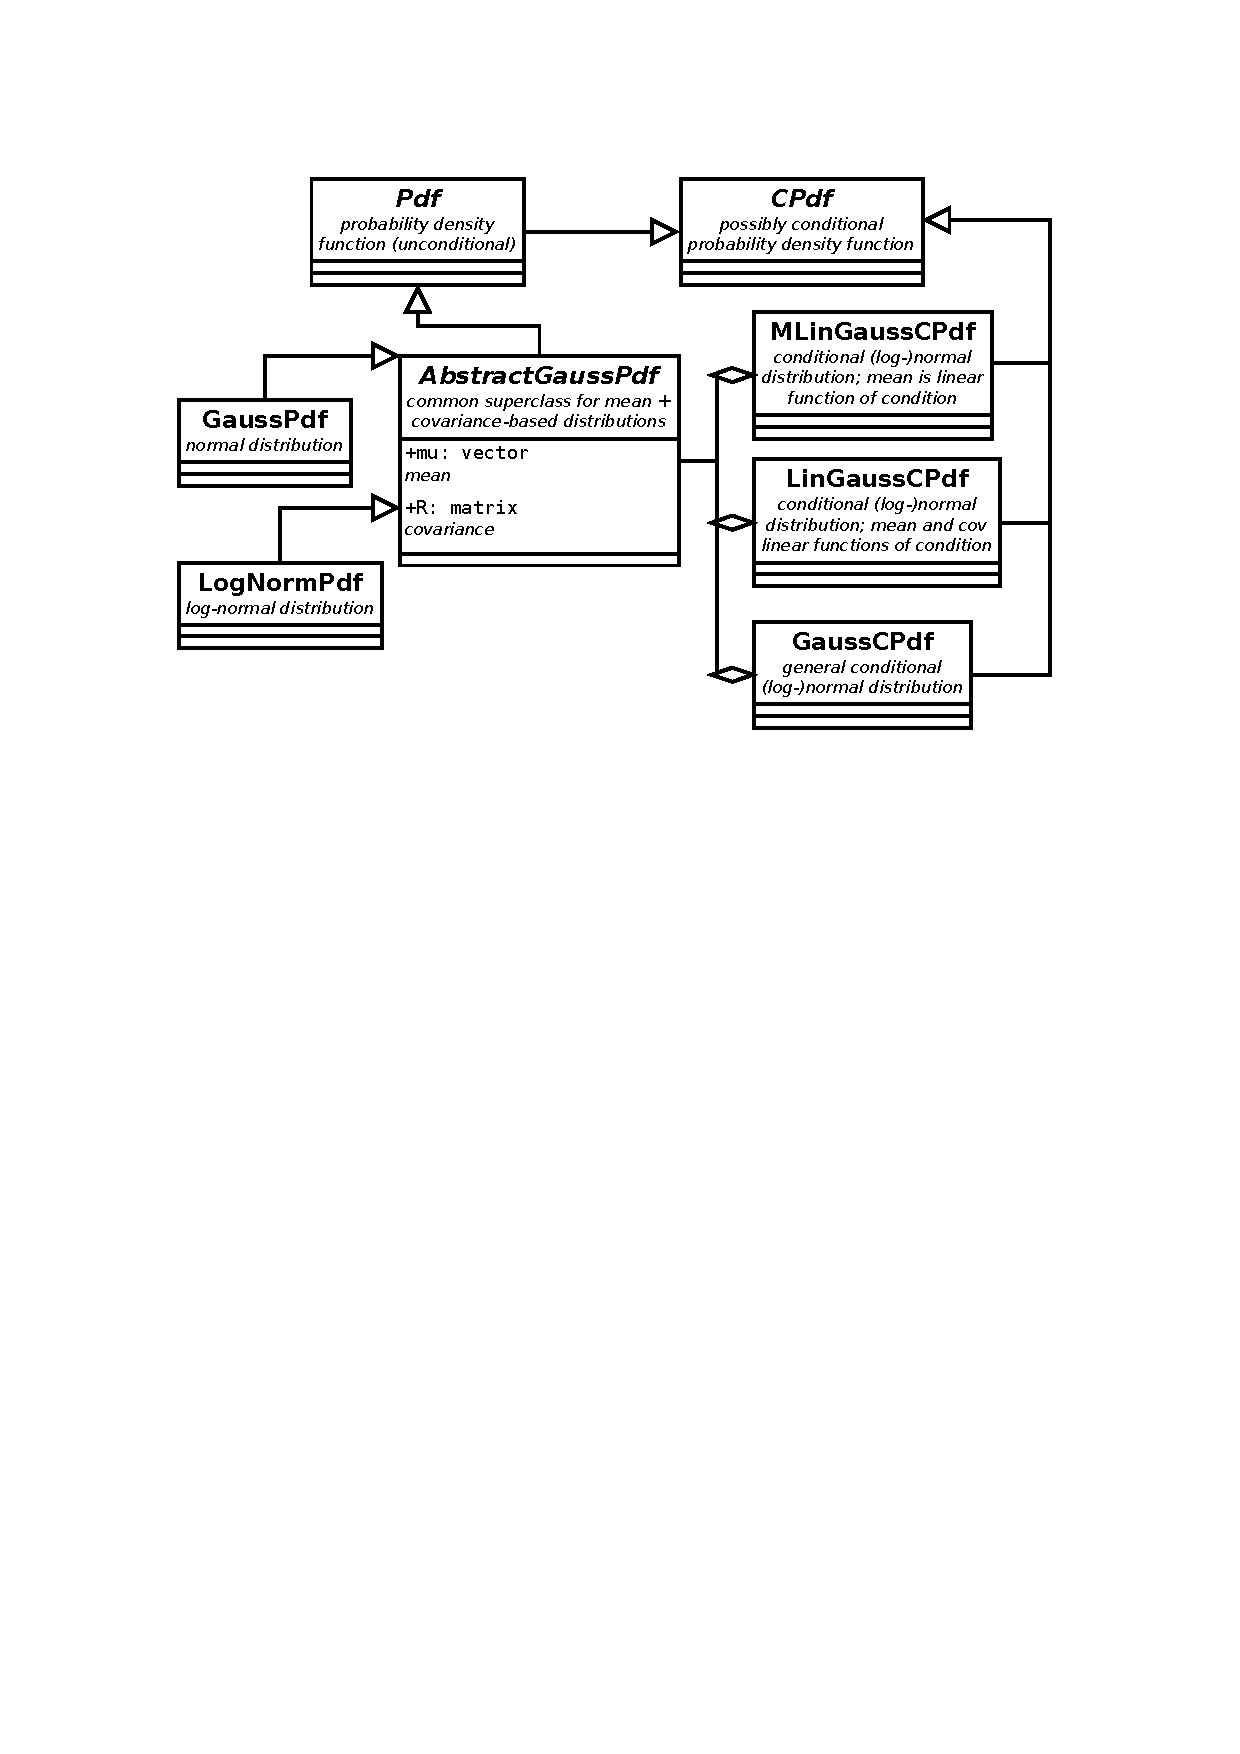
\includegraphics[width=\textwidth,keepaspectratio=true,clip=true,trim=3cm 173mm 3cm 3cm]{./diagrams/gaussian_pdfs.pdf}
	\vspace{-8mm}
	\caption{Class diagram of Gaussian and related distributions}
	\label{fig:DiaGaussPdfs}
\end{figure}

\subsection{Empirical Probability Density Functions}

Another very useful set of distributions is the empirical family suitable for particle filters.
Weighted empirical distribution named EmpPdf in PyBayes is the posterior {\pdf} of the
particle filter while a special product of weighted empirical distribution and a mixture of Gaussian
distributions is the posterior {\pdf} of the marginalized particle filter and is thus named
MarginalizedEmpPdf. Both inherit from AbstractEmpPdf in order to reuse code. Neither of the empirical
densities implement \verb|eval_log()| or \verb|sample()| --- while the latter would be possible, we
are yet to find a valid use-case for it (resampling particles being implemented differently).

The \emph{AbstractEmpPdf} class holds the \verb|weights| parameter, a vector of particle weights denoted as
\(\omega = (\omega_1, \omega_2, \dotsc, \omega_n)\) in formulas. The usual constraints
\eqref{eq:AbstractEmpPdfConstraints} must hold. A simple method \verb|normalise_weights()| normalises
weights according to \eqref{eq:AbstractEmpPdfNormalise}.
\begin{align}
	\omega_i >= 0 \quad \forall i \quad \quad & \quad \quad \sum_{i=1}^n \omega_i = 1 \label{eq:AbstractEmpPdfConstraints} \\
	\omega_i' &= \frac{\omega_i}{\sum_{i=1}^n \omega_i} \label{eq:AbstractEmpPdfNormalise}
\end{align}
AbstractEmpPdf provides one more method called \verb|get_resample_indices()| that
(given that there are \(n\) particles) draws \(n\) random samples from itself and returns their
indices. The algorithm is however optimised in a way that only one random sampling is performed; the
results are thus more predictable (or, ``less random''), but this is desired when used for resampling
in particle filters --- its primary (and currently only) use.

The \emph{EmpPdf} class is the standard weighted empirical distribution \eqref{eq:EmpPdf} that extends
AbstractEmpPdf with the \verb|particles| attribute (a matrix) where each row \(x^{(i)}\) represents
one particle. It also provides the \verb|resample()| method that resamples particles using
\verb|get_resample_indices()| and resets weights to be uniformly distributed. EmpPdf has an extra
role in PyBayes, it is used to test \verb|sample()| of other {\pdfs} using the moment method
(sufficient number of samples is generated and sample mean and variance is compared with theoretical
results).
\begin{equation} \label{eq:EmpPdf}
	p(x) = \sum_{i=1}^n \omega_i \delta(x - x^{(i)})
\end{equation}

Related to the empirical density is the \emph{MarginalizedEmpPdf} that exists solely to form the
posterior {\pdf} of the marginalized particle filter. It extends AbstractEmpPdf with a vector of
GaussPdf objects \verb|gausses|, i-th GaussPdf is denoted as \(\mathcal{N}\left(\hat{a}^{(i)},
P^{(i)}\right)\) and a matrix \verb|particles| where i-th row is denoted as \(b^{(i)}\) in
\eqref{eq:MarginalizedEmpPdf}.
\begin{equation} \label{eq:MarginalizedEmpPdf}
	p(a, b) = \sum_{i=1}^n \omega_i \Big[ \mathcal{N}\left(\hat{a}^{(i)}, P^{(i)}\right) \Big]_a
		\delta(b - b^{(i)})
\end{equation}

MarginalizedEmpPdf doesn't provide a method for resampling as this task have to be done in the
particle filter implementation anyway at it has to deal also with the Kalman filters.

The class diagram of empirical {\pdfs} and related is displayed in the \autoref{fig:DiaEmpPdfs}.

\begin{figure}[ht]
	\centering
	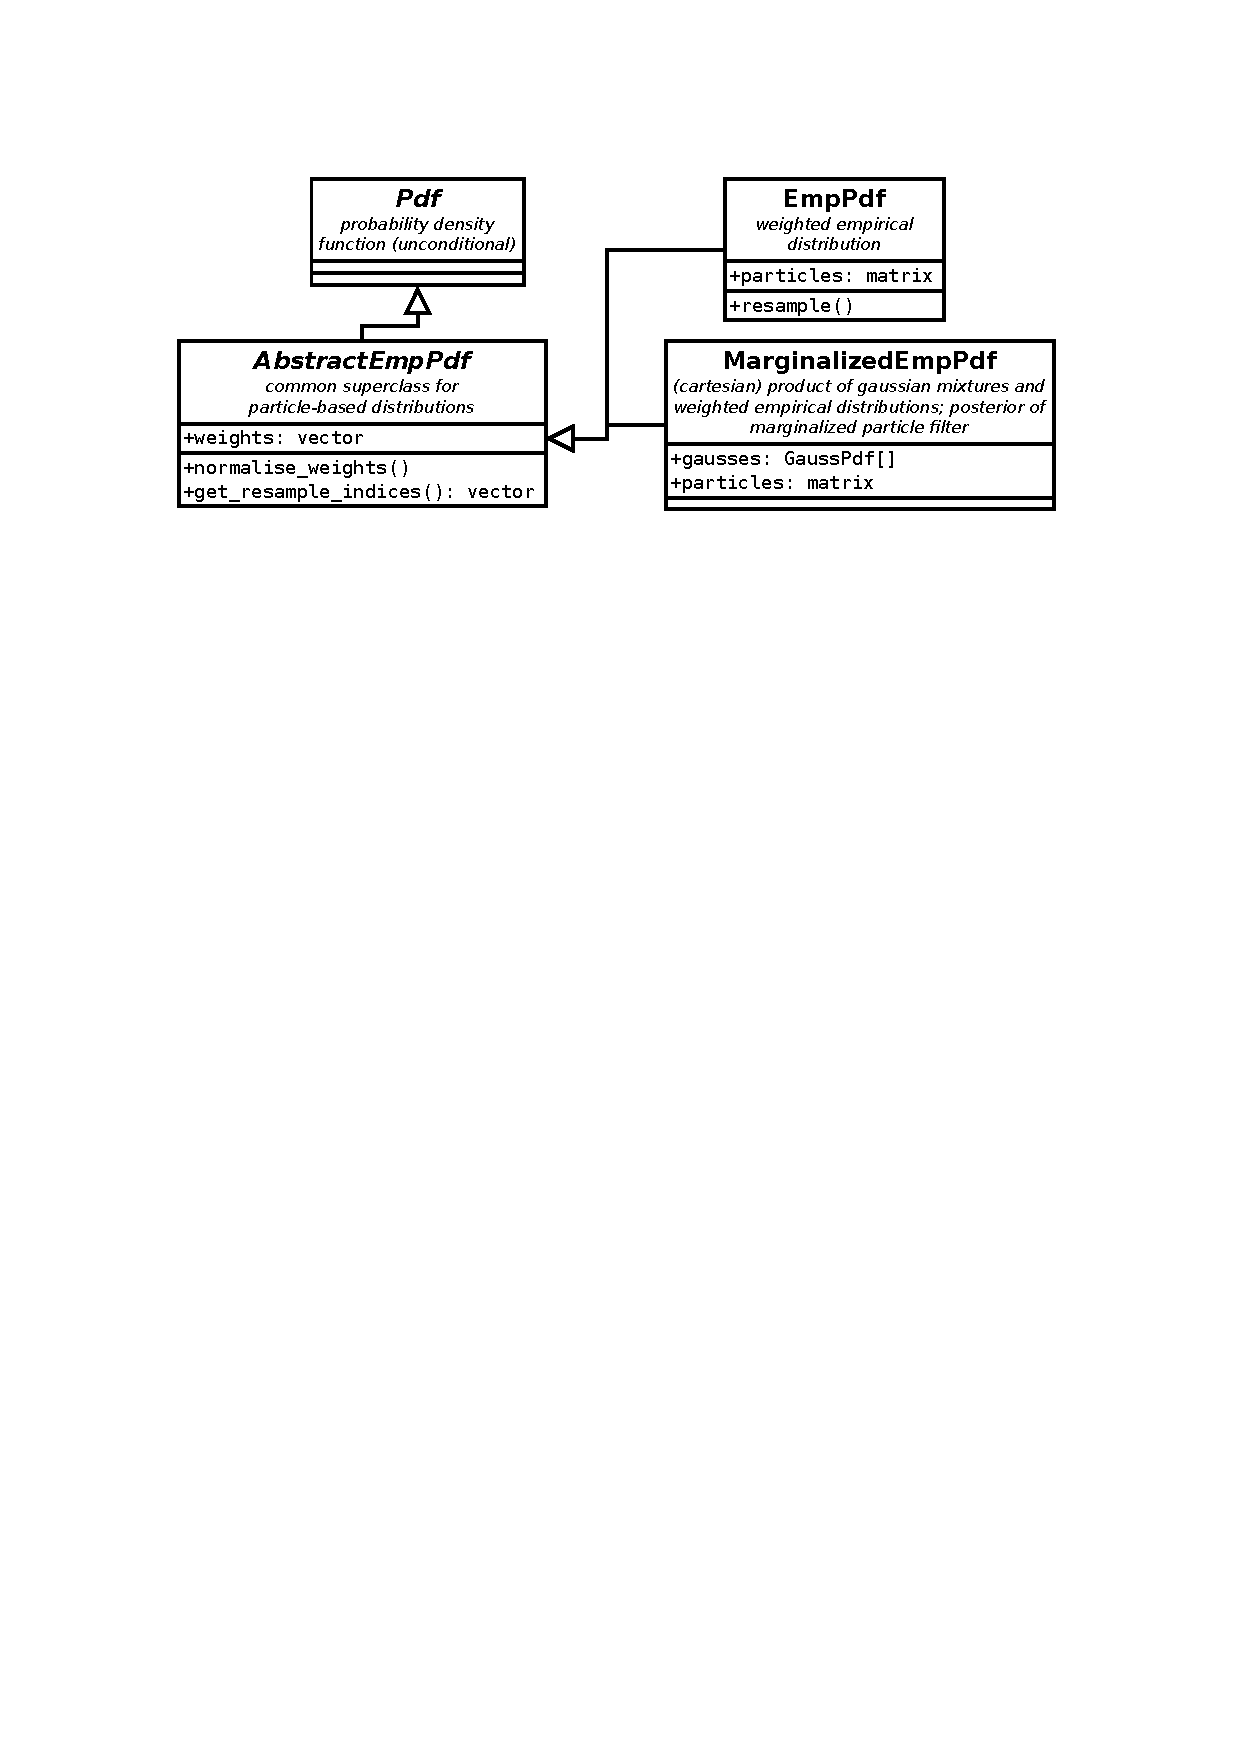
\includegraphics[width=\textwidth,keepaspectratio=true,clip=true,trim=3cm 210mm 3cm 3cm]{./diagrams/emp_pdfs.pdf}
	\vspace{-8mm}
	\caption{Class diagram of empirical distributions}
	\label{fig:DiaEmpPdfs}
\end{figure}

\subsection{Other Probability Density Functions}

We conclude the discussion about the implemented {\pdfs} with the ones that don't fit elsewhere.

The \emph{ProdPdf} class represents unconditional product of \(n\) independent random variables
\(x_1, x_2, \dotsc, x_n\) as depicted in \eqref{eq:ProdPdf}. As an exception from the general rule,
ProdPdf constructs its random variable association (the \verb|rv| attribute) using factor random
variables for convenience; it however currently doesn't make any use of the random variable
meta-representation as it would be of limited usability --- only permutation of random variable
components within \(x_i ~ (\forall i)\) would be additionally possible (the order of factors is
already specified by the user. ProdPdf implements all abstract methods of Pdf by delegating work to
factor {\pdfs}.
\begin{equation} \label{eq:ProdPdf}
	p(x_1, x_2, \dotsc, x_n) = p_1(x_1) p_2(x_2) \dotsm p_n(x_n)
\end{equation}

A more sophisticated variant of the ProdPdf is the \emph{ProdCPdf} class that is potentially
conditional and allows for conditionally dependent random variables. In general it can represent
a~chain rule for
{\pdfs} shown in \eqref{eq:ProdCPdf} with an additional constraint that the right hand side makes
sense (that means that there exists a sequence \((p_{j_1}, p_{j_2}, \dotsc, p_{j_m})\) for which
\eqref{eq:ProdCPdfContraint} holds). The relation ``\(C \subset \{x_i, x_j, x_k, \dotsc\}\)'' denotes
``random variable \(C\) is composed of the (subset of) \(x_i, x_j, x_k, \dotsc\) random variable components''
in the following formulas.
\begin{gather} \label{eq:ProdCPdf}
	\begin{gathered}
		p(x_1, x_2, \dotsc, x_m | x_{m+1}, x_{m+2} , \dotsc, x_n) = p_1(x_1 | C_1)
			p_2(x_2 | C_1) \dotsm p_m(x_m | C_m) \\
		\text{where} \quad m \leq n; \quad
			\forall i \in \{1, 2, \dotsc, m\}: C_i \subset \{x_1, x_2, \dotsc, x_n\}
	\end{gathered}
\end{gather}
\begin{equation} \label{eq:ProdCPdfContraint}
	\forall k \in \{1, 2, \dotsc, m\}: C_{j_k} \subset \{x_1, x_2, \dotsc, x_{k-1}\} \cup \{x_{m+1}, x_{m+2} , \dotsc, x_n\}
\end{equation}

As in ProdPdf, all abstract methods of CPdf are implemented.
ProdCPdf makes extensive use of the random variable meta-representation described earlier; it uses
random variable descriptions of factor densities \(p_1, p_2, \dotsc, p_m\) to construct the
data-flow (the \((p_{j_1}, p_{j_2}, \dotsc, p_{j_m})\) sequence); the order of passed factor
distributions is therefore insignificant --- ProdCPdf always computes correct evaluation order if
it exists. For this reason the random variable components of factor {\pdfs} need to be specified
(at least those that are ``shared'' between multiple factor distributions). Currently, there is also
a limitation that compound random variable representations have to be additionally passed to ProdCPdf;
in future, ProdCPdf will be able to infer compound random variables from factor distributions.
Following code example constructs a simple {\pdf} from \eqref{eq:ProdCPdfSimple}:
\begin{equation} \label{eq:ProdCPdfSimple}
	p(a,b) = p_1(a|b) p_2(b)
\end{equation}

\begin{Verbatim}[samepage=true,gobble=1,label=ProdCPdf example,frame=single]
	# prepare random variables:
	a, b = RVComp(m, "name of a"), RVComp(n, "b name")
	p_1 = SomeCPdf(..., rv=RV(a), cond_rv=RV(b))
	p_2 = OtherPdf(..., rv=RV(b))
	p = ProdCPdf((p_1, p_2), rv=RV(a, b), cond_rv=RV()) # empty cond_rv

	# version 0.4 of PyBayes will allow:
	p = ProdCPdf((p_1, p_2))
\end{Verbatim}
PyBayes also provides a multivariate uniform distribution which is implemented by the \emph{UniPdf}
class.

\subsection{Bayesian Filters}

Bayesian filters are the \emph{raison d'être} of PyBayes. It turned out however that with a solid
framework of {\pdfs}, their implementation is rather straightforward. All filters in PyBayes extend
an abstract class \emph{Filter} that acts as a prototype of all filters. Filter defines following
methods that can/should be implemented by subclasses:
\begin{itemize}
	\item \verb|bayes(yt : vector, cond : vector = None)| \\
		compute posterior {\pdf} given
		the observation \verb|yt|; semantics of the optional \verb|cond| parameter are defined
		by filter implementations. The method name comes from the fact that computing the posterior
		{\pdf} involves applying (exact or approximate) Bayes rule; see \eqref{eq:PosteriorPdfRaw}
		on page \pageref{eq:PosteriorPdfRaw}.
	\item \verb|posterior() : Pdf| \\
		return a reference to the posterior {\pdf} \(p(x_t | y_{1:t})\) \eqref{eq:PosteriorPdf}
		(p.~\pageref{eq:PosteriorPdf}).
	\item \verb|evidence_log(yt : vector) : float| \\
		return logarithm of the marginal likelihood \(p(y_t | y_{1:t-1})\) \eqref{eq:MargLikelihood}
		(p.~\pageref{eq:MargLikelihood}) evaluated in point \verb|yt|. Subclasses may choose not to
		implement this method if it is not feasible.
\end{itemize}
Fists subclass of Filter is the \emph{KalmanFilter} class that implements slightly extended version
of the Kalman filter presented in the first chapter --- KalmanFilter can optionally accept control
vector in its \verb|bayes| method (passed through the \verb|cond| parameter) making it suitable also
for the theory of Bayesian decision-making.

Speaking about the particle filter family, it has been suggested in \cite{Smi:10} that the particle
filter and the marginalized particle filter can be merged into one general class using a recursive
structure of classes representing the Bayes rule (e.g. Filter in PyBayes). This approach has not
been used in PyBayes for performance and simplicity reasons. On the other hand, particle filters in
PyBayes offload much work to {\pdfs} in PyBayes where code is reused thanks to AbstractEmpPdf.

The \emph{ParticleFilter} class implements a simple version of the particle filter as presented in
the first chapter. ParticleFilter takes the process model \(p(x_t|x_{t-1})\) and the observation
model \(p(y_t|x_t)\) distributions in constructor (along with the initial density and number of
particles) and employs \verb|resample()| and \verb|normalise_weights()| of the EmpPdf class that it
uses for the posterior distribution. ParticleFilter currently doesn't support specifying the
proposal density, although it is planned in future.

\begin{figure}[h!]
	\centering
	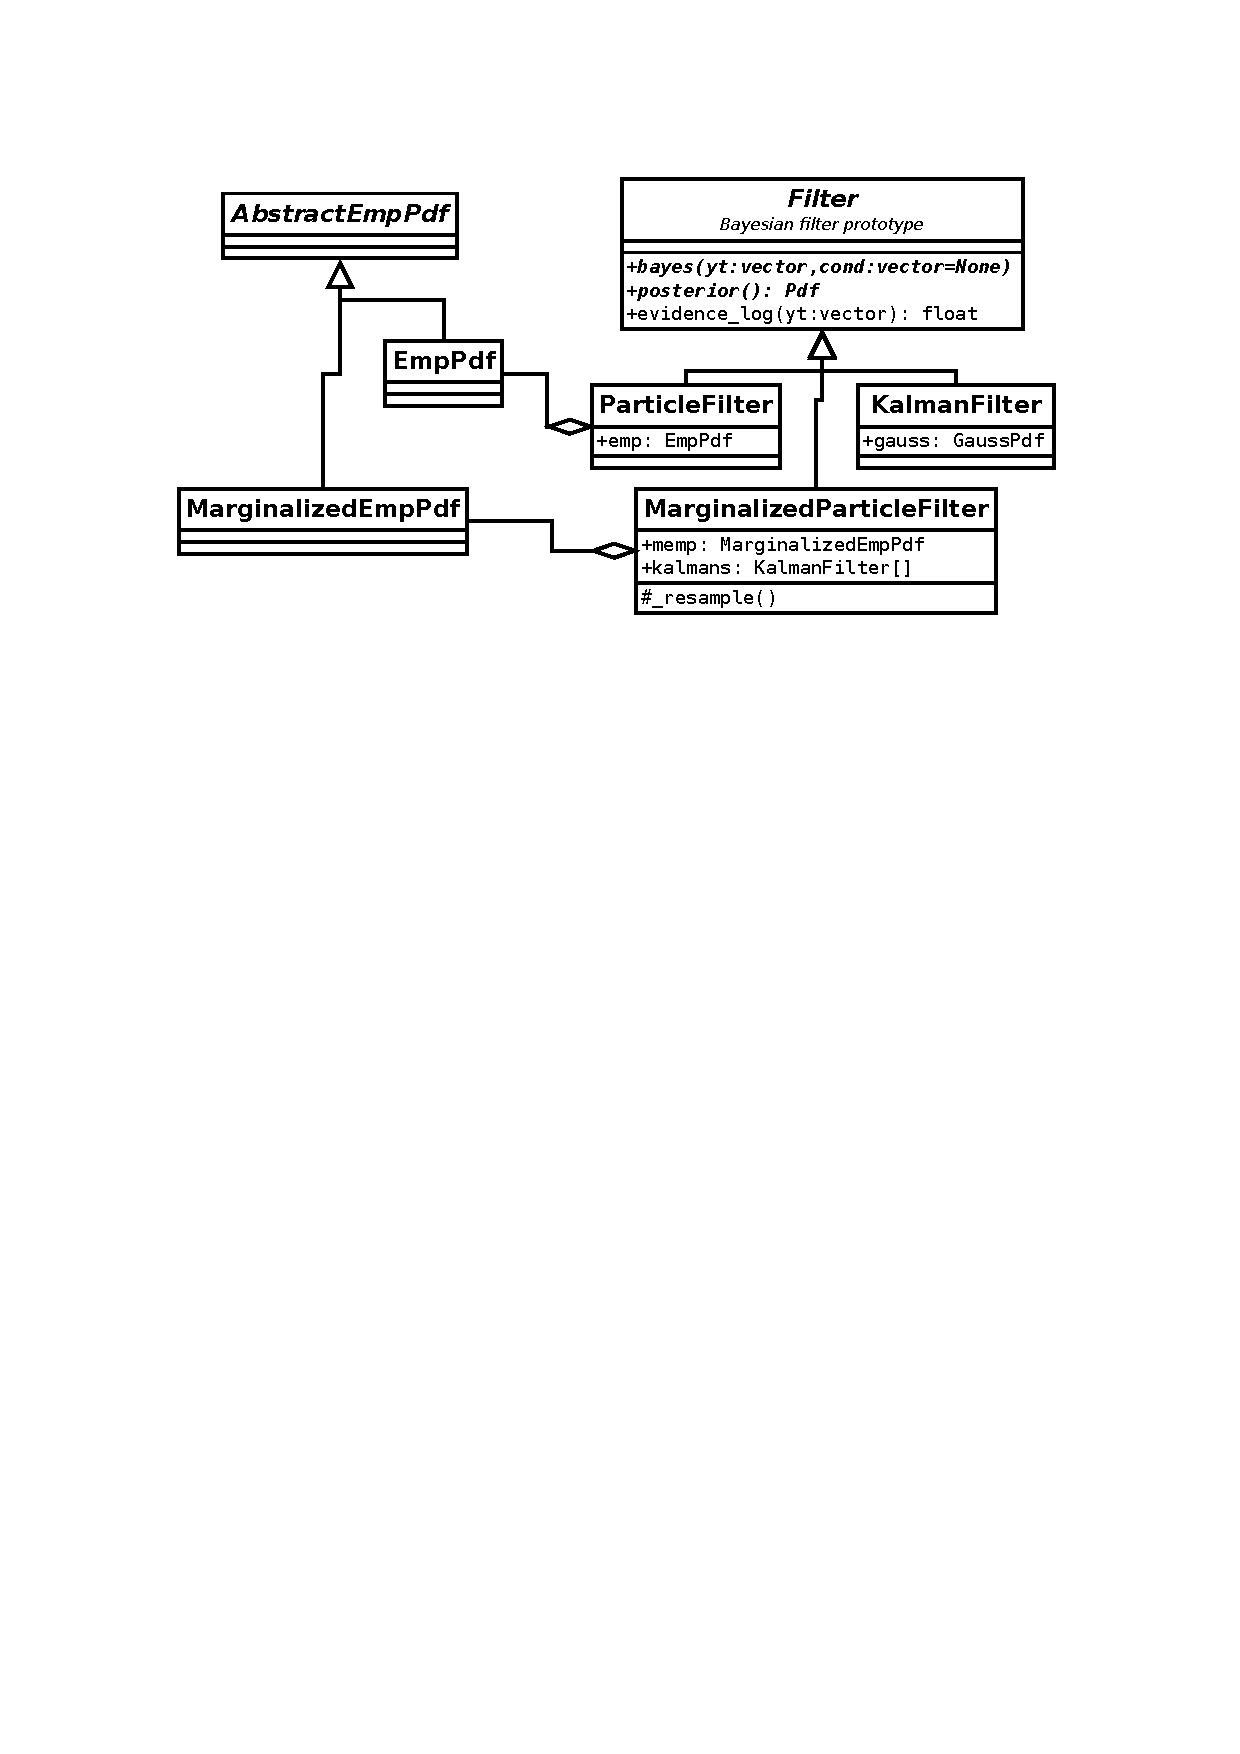
\includegraphics[width=\textwidth,keepaspectratio=true,clip=true,trim=3cm 192mm 3cm 3cm]{./diagrams/filters.pdf}
	\vspace{-8mm}
	\caption{Class diagram of Bayesian filters}
	\label{fig:DiaFilters}
\end{figure}

\emph{MarginalizedParticleFilter} also implements the respective algorithm shown in the first
chapter and offloads some work to its posterior {\pdf}, MarginalizedEmpPdf, but has to provide its
own array of KalmanFilter objects. The MarginalizedParticleFilter class ensures that the i-th Kalman
filter shares its posterior Gaussian distribution with MarginalizedEmpPdf's i-th particle. This is
the reason why resampling cannot be done in MarginalizedEmpPdf and is instead performed in the
\verb|_resample()| method of MarginalizedParticleFilter that makes use of the
\verb|get_resample_indices()| method of AbstractEmpPdf.

In constructor MarginalizedEmpPdf accepts initial distribution of the state vector
\(p(x_0) = p(a_0, b_0)\), process model of the empirical part of the state vector \(p(b_t|b_{t-1})\),
the class of the desired Kalman filter implementation (that has to be a subclass of KalmanFilter)
and its parameters in form of a Python dictionary. That way, thanks to Python capabilities,
MarginalizedEmpPdf will support other variants of the Kalman filter in future without a need to be
changed. It also means that the observation model is specified using the Kalman filter implementation
and parameters for it, which makes MarginalizedParticleFilter more flexible. The process model is
given by the combination of \(p(b_t|b_{t-1})\) and supplied Kalman filter implementation (and its
parameters). Current implementation hard-codes \(b_t\) to be the observation and process noise of
the modelled system; this silly limitation will be lifted in future where MarginalizedParticleFilter
will pass the \(b_t\) vector as the \verb|cond| argument to the \verb|bayes()| method of the
specified Kalman filter implementation.

A diagram of filtering classes in shown in the \autoref{fig:DiaFilters}.

\subsection{Wrappers} \label{sec:PyBayesWrappers}

Favourable performance was one of the criteria for the desired library for Bayesian filtering. When
the performance of the KalmanFilter class was benchmarked with a small system (both state and
observation vectors were 2-dimensional); it was discovered that a great portion of total run time
was spent in the boilerplate code of NumPy functions \verb|dot()| (for matrix product) and
\verb|inv()| (for matrix inversion). Even though NumPy uses BLAS and LAPACK internally, the time
spent in the intermediate Python code was unacceptable (it was probably made more visible due to
the small size of the system); see the \autoref{sec:CythonFeatures} on page
\pageref{sec:CythonFeatures} for information about Cython \(\leftrightarrow \) NumPy co-operation.

Fortunately, a project that approaches popular BLAS and LAPACK functions more directly was found:
Shane Legg's Tokyo\footnote{\url{http://www.vetta.org/2009/09/tokyo-a-cython-blas-wrapper-for-fast-matrix-math/}}
wraps BLAS (and a couple of LAPACK) procedures in Cython using NumPy's \verb|ndarray| data-type.
Quick tests have shown great speed-ups --- the mentioned functions ceased to be performance
bottle-necks. It was therefore decided that the Tokyo project should be used in the Cython mode of
PyBayes and it was forked\footnote{\url{https://github.com/strohel/Tokyo}} on github to provide
a~couple of bug-fixes we made to the public. For convenience, Tokyo is also bundled with PyBayes
releases and is built along it to reduce dependencies on obscure libraries.

A special approach in PyBayes has been taken in order to support both Python and
Cython mode: wrapper modules for \verb|numpy| and \verb|numpy.linalg| were created in the
\verb|pybayes.wrappers| package; Python versions of the wrappers (.py files) just import appropriate
NumPy modules. Cython versions do nearly the same, but provide own implementations (that call Tokyo)
of the offending NumPy functions (and delegate the rest to NumPy). Other code then imports
\verb|wrappers._numpy| instead of \verb|numpy|, likewise for \verb|numpy.linalg|.

\section{Documentation and Testing} \label{sec:PyBayesDocsTests}

Second pillar of each well-written software library is, in our belief, its \emph{documentation}; the
first one being the library design and the actual implementation being no better than the third
pillar (in our view, the implementation can be easily modified in a well-designed library). PyBayes
reflects that and puts great emphasis on the API Documentation, that is
\ifattachements included on the bundled CD-ROM and \fi
accessible on-line at \url{http://strohel.github.com/PyBayes-doc/}.

Documentation is generated almost solely from the documenting comments --- Python ``Docstrings'' as
defined in PEP 257,\footnote{Python Enhancement Proposal 257: \url{http://www.python.org/dev/peps/pep-0257/}}
using the Sphinx Python documentation generator.\footnote{\url{http://sphinx.pocoo.org/}} Sphinx
supports additional syntax in Docstrings and is able to generate documentation in a wide range of
formats including HTML, Qt Help,\footnote{\url{http://doc.qt.nokia.com/qthelp-framework.html}}
Devhelp,\footnote{\url{http://live.gnome.org/devhelp}} \LaTeX, PDF, man-pages and many others. One
very valuable feature of Sphinx is the ability to parse {\LaTeX}-encoded mathematics embedded
directly into Docstrings; these are then rendered to images in HTML output for example.

Every publicly available class and method in PyBayes is extensively documented and enhanced with
mathematical formulas where appropriate. We believe that this approach makes
PyBayes more easily usable by mathematicians and eliminates any possible misunderstanding of the textual
description of classes and methods. An example of how Docstrings look like in code can be seen in
the \autoref{fig:Coverage}. We must say we are very satisfied with Sphinx can only recommend using
it.

As noted in the discussion about dynamically-typed languages, almost all programmer errors in such
languages are only discovered at runtime, therefore a need for a comprehensive test-suite was
stressed out. PyBayes follows this advice and provides two packages that accomplish testing:
\begin{itemize}
	\item \verb|pybayes.tests| \\
		package contains unit-tests of virtually all PyBayes classes and methods. Unit-testing
		evaluates classes and methods \emph{in isolation} (to highest possible extent) and therefore
		forms an excellent tool for finding precise location of possible bugs. Unit-testing should
		last no longer than a few seconds so that it can be run on per-commit basis. One problem
		faced in PyBayes are non-deterministic methods such as \verb|CPdf.sample()| or
		\verb|bayes()| methods of particle filters. \verb|sample()| methods are currently tested
		by generating high enough number of particles and then comparing their mean and variance
		with theoretical values.
		Another option would be mocking the random number generator to force deterministic results,
		this could however produce false-positives when an implementation of a given \verb|sample()|
		method changed.

		PyBayes currently contains 99 unit-tests that run in approximately 0.2 seconds.
	\item \verb|pybayes.stresses| \\
		package contains so-called stress-tests --- longer-running procedures that test greater
		portion of code and cooperation if individual modules. Results of stresses are not intended
		be checked automatically, they rather require human evaluation. PyBayes currently has three
		stresses, one for each Bayesian filter implementation, that are run with various parameters
		to ensure that the filters produce valid-looking results, to measure their performance, and
		(for particle filters) to test their convergence as the number of particles increases.
\end{itemize}
To ensure that all code-paths are properly tested, it is advisable to employ a \emph{code coverage}
tool that shows which code statements were visited during tests. We've used Ned Batchelder's excellent
\emph{coverage.py}\footnote{\url{http://nedbatchelder.com/code/coverage/}} to discover that 86\%
statements in the \verb|pdfs| module and 83\% statements in the \verb|filters| module are covered
by tests and stress-tests combined. An example output of coverage.py is shown in the
\autoref{fig:Coverage}, where everything except one code-path throwing an exception is covered by
a test.

\begin{figure}[ht]
	\centering
	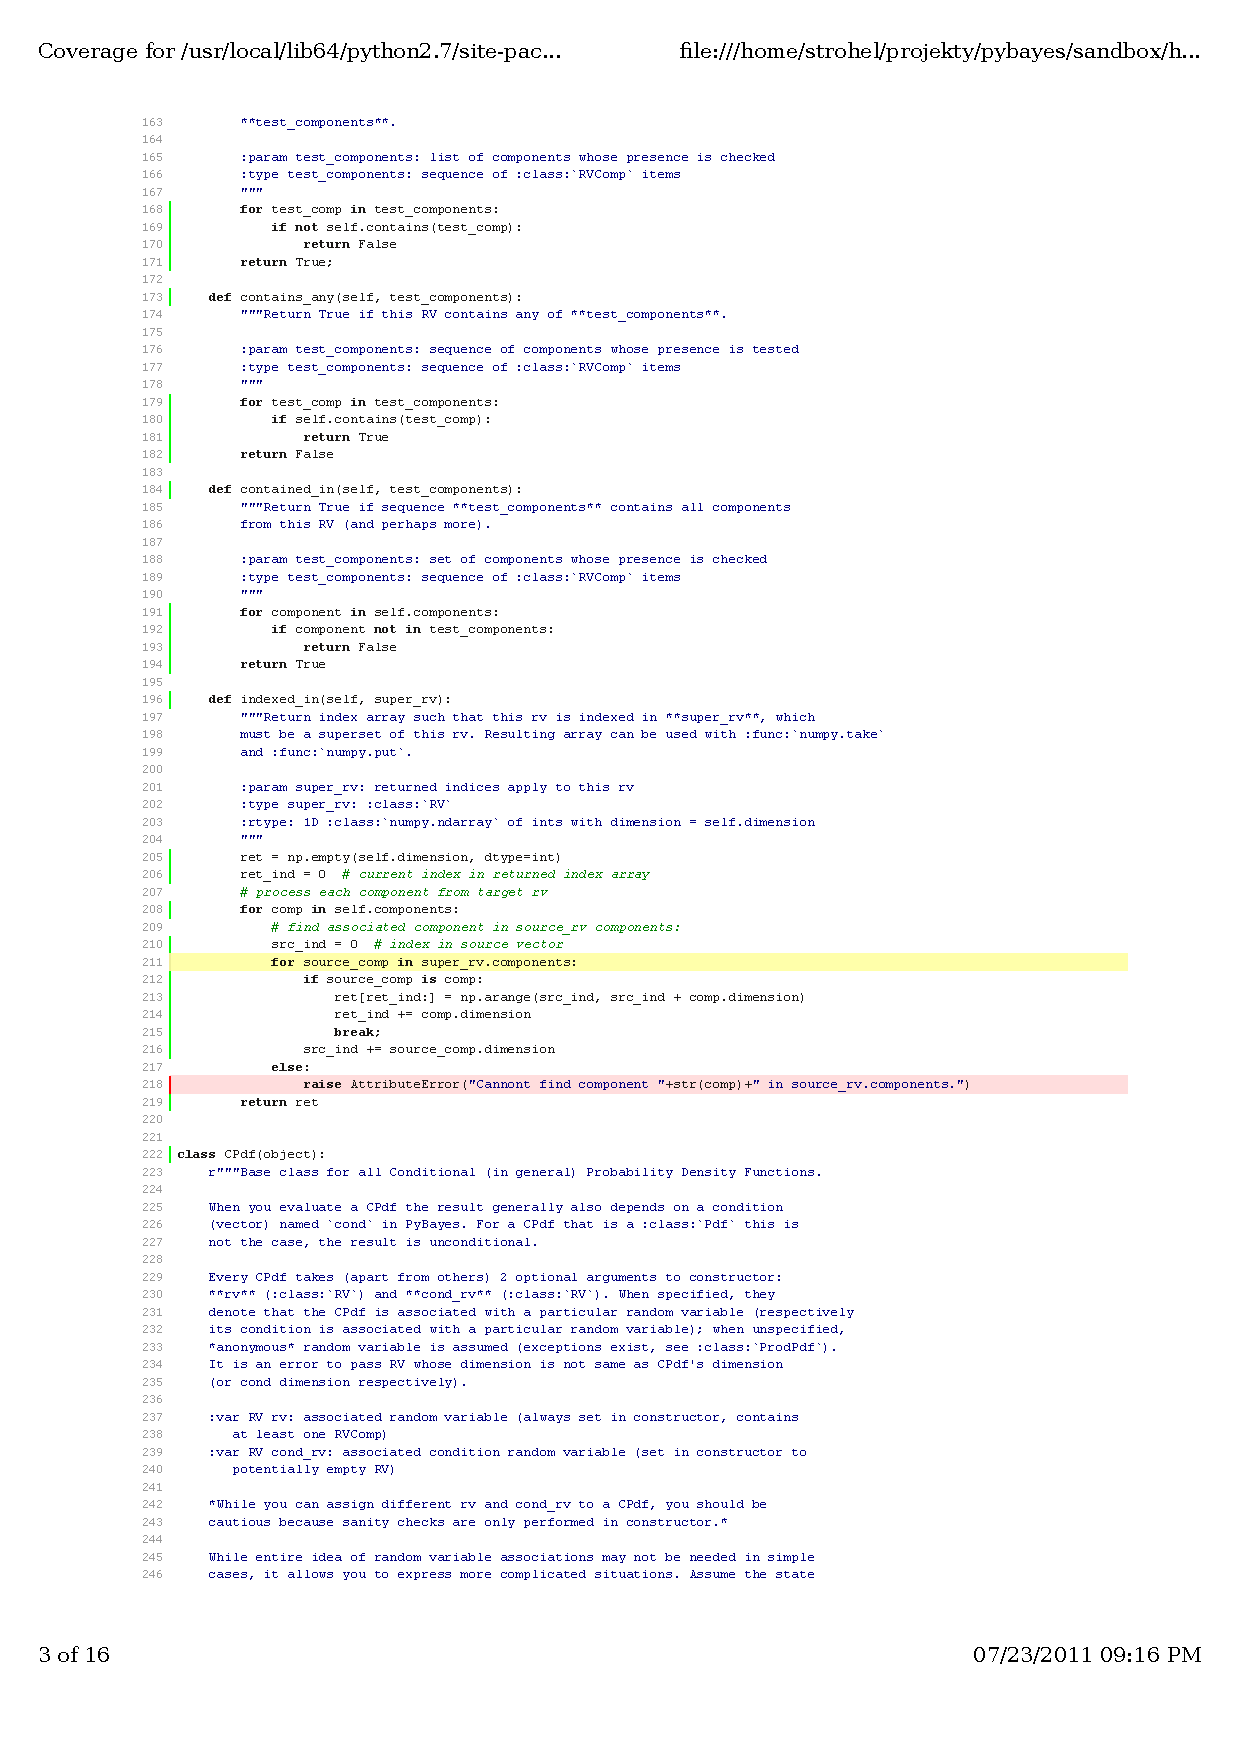
\includegraphics[width=\textwidth,keepaspectratio=true,clip=true,trim=24mm 109mm 60mm 117mm]{./coverage.pdf}
	\vspace{-8mm}
	\caption{coverage.py shows that one code-path in indexed\_in() is uncovered}
	\label{fig:Coverage}
\end{figure}

\section{Performance Comparison with BDM} \label{sec:PyBayesPerformance}

The chapter about the PyBayes library is concluded by a benchmark of four various Kalman filter
implementations from PyBayes and BDM~\cite{BDM}. All tested implementations use exactly the same
algorithm and equivalent data-types, neither is explicitly parallelised (however, see notes about
MATLAB), operate on the same data and gave exactly the same results as shown in the \autoref{fig:KF}
on page \pageref{fig:KF}. Following versions of involved software were used:
\begin{description}
	\item[Python] 2.7.1
	\item[GNU C Compiler] 4.4.5; \verb|-O2| optimisation flag used when compiling C files
	\item[Cython] 0.14.1+ (git revision 0.14.1-1002-g53e4c10)
	\item[MATLAB] 7.11.0.584 (R2010b) 64-bit (glnxa64)
	\vspace{1mm}
	\item[PyBayes] 0.3
	\item[BDM] SVN revision r1378
\end{description}

The test was performed on a 64-bit dual-core Intel Core i5-2520M CPU clocked at 2.50 Ghz with Intel Turbo
Boost and Hyper-threading enabled; operating system is Gentoo Linux compiled for the x86\_64 platform.

The test consists of running 3000 iterations of the Kalman filter with various state-space dimensions:
2, 30 and 60; observation vector is has the same dimensionality as the state vector. Wall-clock time
needed to complete all iterations is measured. Each implementation was tested 10 times, mean values
are shown; to measure variance across runs, relative sample standard deviation \(s_{\text{rel}}\)
computed using \eqref{eq:RelStdDev} (page \pageref{eq:RelStdDev}) was measured. Additionally,
relative speed-up with regards to reference version \textbf{PyBayes Cy} is displayed for
illustration. Following versions of Kalman filter/implementation environments were under test:
\begin{description}
	\item[PyBayes Py] \hfill \\
		KalmanFiler class from PyBayes \url{pybayes/filters.py}; Python build
	\item[PyBayes Cy] \hfill \\
		KalmanFiler class from PyBayes \url{pybayes/filters.py}; Cython build
	\item[MATLAB imper.] \hfill \\
		Imperative MATLAB implementation where the whole algorithm is written
		in a single for loop; comes from BDM, file \url{library/tests/stressuite/kalman_stress.m}.
		While not explicitly parallelised, later experiments shown that MATLAB implicitly
		parallelised the code behind curtain at least in higher-dimensional cases.
	\item[MATLAB o-o] \hfill \\
		Object-oriented MATLAB implementation from BDM where the filter and Gaussian {\pdf} is
		represented using MATLAB classes; file \url{applications/bdmtoolbox/mex/mexKalman.m}.
	\item[BDM] \hfill \\
		 Object-oriented C++ class KalmanFull from BDM implemented in
		 \url{/library/bdm/estim/kalman.cpp}.
\end{description}
Benchmark results are shown in tables \ref{tab:KFSmall} to \ref{tab:KFHuge}. The greatest variance
in results is achieved in a small (2-dimensional) system, where the C++ version is the fastest,
outperforming Cython build of PyBayes by 260\%, and object-oriented MATLAB version is embarrassingly
15\x\ slower than the PyBayes Cy.

\begin{table}[ht]
	\centering
	\begin{tabular}{|r|l|l|l|l|l|} \hline
		& PyBayes Py & PyBayes Cy & MATLAB imper. & MATLAB o-o & BDM \\ \hline
		time [s] & 0.254 & 0.091 & 0.069 & 1.378 & 0.026 \\ \hline
		\(s_{\text{rel}}\) & 4.4\% & 4.2\% & 8.5\% & 4.1\% & 9.3\% \\ \hline
		speedup & 0.4\x & 1.0\x & 1.3\x & 0.1\x & 3.6\x \\ \hline
	\end{tabular}
	\caption{Performance of Kalman filters: 2-dimensional state-space}
	\label{tab:KFSmall}
	\vspace{7mm}

	\begin{tabular}{|r|l|l|l|l|l|} \hline
		& PyBayes Py & PyBayes Cy & MATLAB imper. & MATLAB o-o & BDM \\ \hline
		time [s] & 0.689 & 0.535 & 0.424 & 1.780 & 0.518 \\ \hline
		\(s_{\text{rel}}\) & 3.0\% & 5.4\% & 5.9\% & 2.7\% & 5.7\% \\ \hline
		speedup & 0.8\x & 1.0\x & 1.3\x & 0.3\x & 1.0\x \\ \hline
	\end{tabular}
	\caption{Performance of Kalman filters: 30-dimensional state-space}
	\label{tab:KFBig}
	\vspace{7mm}

	\begin{tabular}{|r|l|l|l|l|l|} \hline
		& PyBayes Py & PyBayes Cy & MATLAB imper. & MATLAB o-o & BDM \\ \hline
		time [s] & 2.120 & 1.816 & 1.274 & 3.849 & 1.948 \\ \hline
		\(s_{\text{rel}}\) & 2.4\% & 2.6\% & 6.3\% & 9.9\% & 2.1\% \\ \hline
		speedup & 0.9\x & 1.0\x & 1.4\x & 0.5\x & 0.9\x \\ \hline
	\end{tabular}
	\caption{Performance of Kalman filters: 60-dimensional state-space}
	\label{tab:KFHuge}
\end{table}

Raising the dimensionality of state-space to 30 produced more even results with object-oriented
MATLAB still lagging behind, PyBayes Cy and C++ version from BDM being nearly equal and imperative
MATLAB version taking lead by being approximately 30\% faster.

A huge 60-dimensional system sees PyBayes Py, PyBayes Cy and BDM versions being even closer,
imperative MATLAB version extending its advantage and object-oriented MATLAB version still largely
unusable due to its poor performance.

The chart shown in the \autoref{fig:KFPerf} allows for some speculations about possible reasons
of performance differences. First, it seems that the Python version adds moderate per-statement
overhead that doesn't raise with number of dimensions (we blame NumPy for Python version being
on par with the C++ and Cython versions) while object-oriented MATLAB adds \textbf{enormous} overhead
that worsens slightly with number of dimensions.

The clear advantage of the imperative MATLAB version can be accounted to its capability to parallelise
code behind the scenes, in our belief. Our informal late tests have shown that it performs very
close to the PyBayes Cy version on uniprocessor systems.

\begin{figure}[h!]
	\centering
	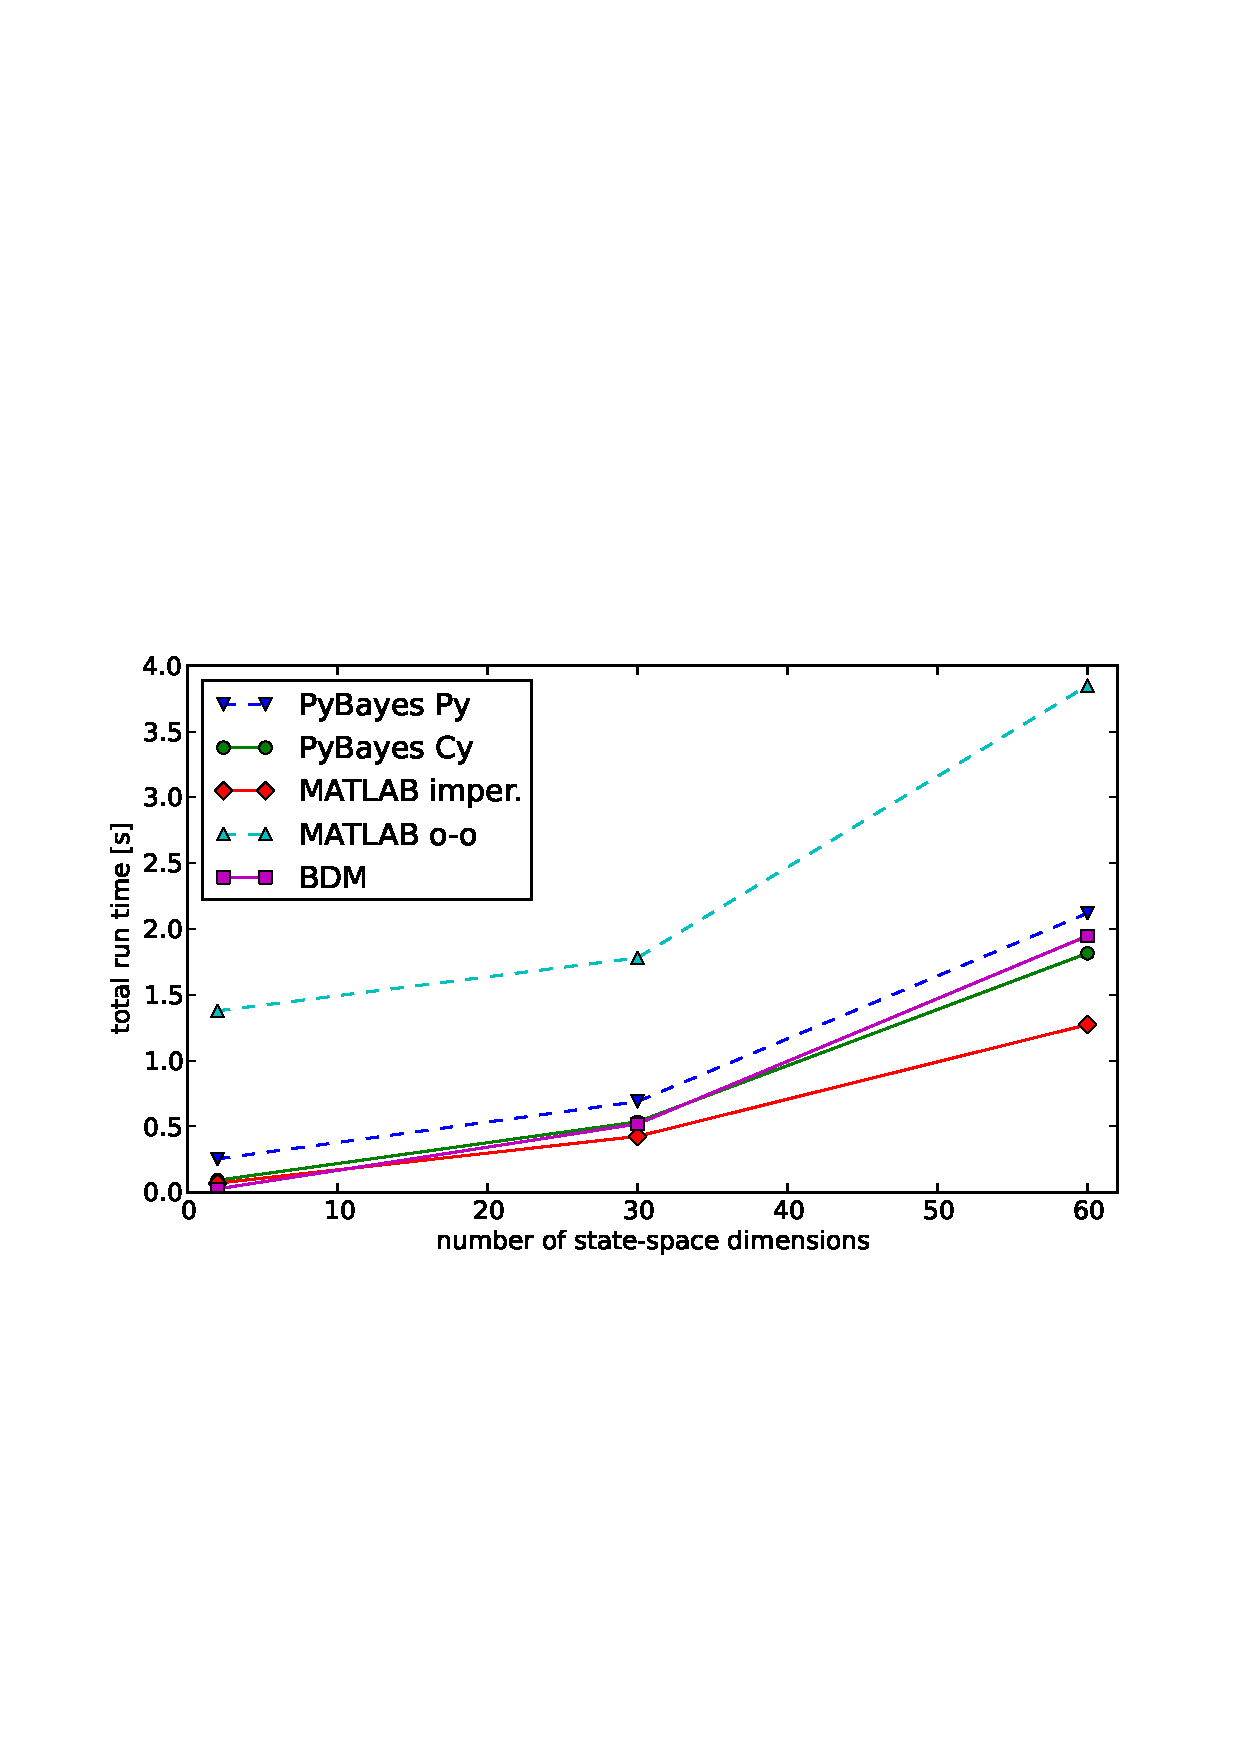
\includegraphics[height=7cm,keepaspectratio=true,clip=true,trim=19mm 85mm 20mm 111mm]{./KFPerf.pdf}
	\caption{Run time against dimensionality of various Kalman filter implementations}
	\label{fig:KFPerf}
\end{figure}
